\chapter{A2}

{\LARGE 'Determine the 50 most popular IP addresses external to the domain by number of flows'}
´
\section{Explicação do código desenvolvido}

A computação deste tópico não apresentou uma dificuldade muito superior em comparação com o tópico anterior, no entanto foi usada uma função auxiliar para facilitar e tornar o código mais legível. A função auxiliar basicamente diz-nos se o endereço IP que estamos a tratar faz parte do domínio ou se é externo. Assim conseguimos com facilidade fazer uma lsita de tuplos onde agrupamos o \textit{IP} com o número de \textit{flows}. Por fim fazemos uma ordenação pela quantidade de flows e descartamos quaisquer resultados após os 50 primeiros. O código seguinte mostra a parte do \textit{script} que trata de cada tuplo do ficheiro.


%TODO
\begin{figure}[h!]
    \label{high}
    \centering
    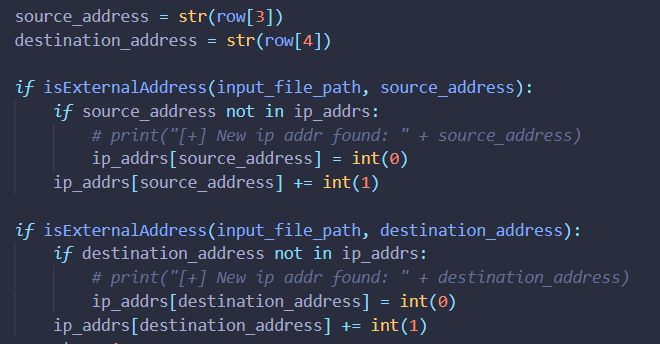
\includegraphics[width=0.8\textwidth]{Images/a2/a2.png}
    \caption{\textit{Código do tópico a2}}
\end{figure}

%----------------------------------------------------------------------------
%----------------------------------------------------------------------------

\newpage

\section{Resulados obtidos pelo ficheiro www.fct.unl.pt.csv}

Como  se  pode  ver  na  figura  3.3,  foram  processadas  as  21362  linhas  do ficheiro www.fct.unl.pt.csv, e foram recolhidos e ordenados os endereços IPs com maior número de flows.

\begin{figure}[h]
    \label{high}
    \centering
    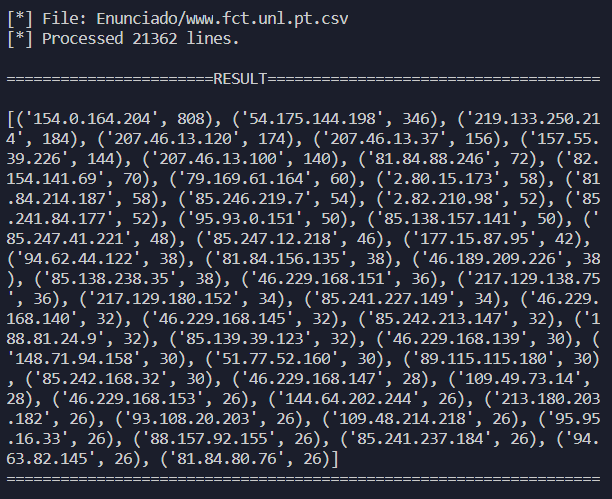
\includegraphics[width=0.9\textwidth]{Images/a2/a2_a.png}
    \caption{\textit{Output do script a2.py}}
\end{figure}

\newpage

%----------------------------------------------------------------------------

\section{Resulados obtidos pelo ficheiro bigFlows.csv}

Na figura 3.4 verificamos que foram processadas 42845 linhas do ficheiro bigFlows.csv, e foram recolhidos e ordenados os endereços IPs com maior número de flows. Fique de notar a diferença na quantidade de flows recolhida.

\begin{figure}[h]
    \label{high}
    \centering
    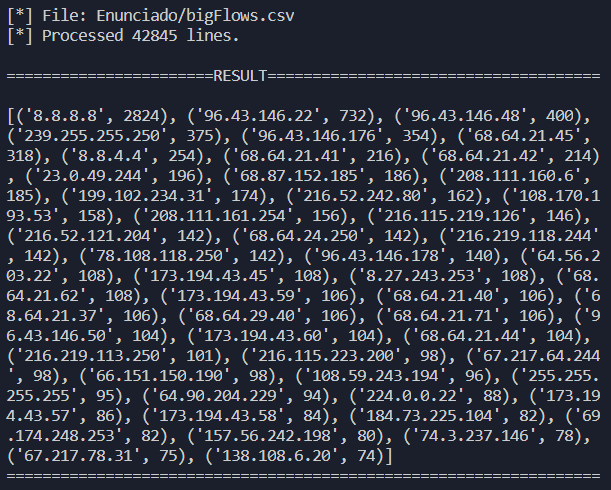
\includegraphics[width=1\textwidth]{Images/a2/a2_b.png}
    \caption{\textit{Output do script a2.py}}
\end{figure}
